\documentclass{beamer}
\usetheme{ConnectivityLab}
\usepackage{times}
\usepackage{graphicx}
\usepackage{verbatim}
\usepackage{outlines}
\usepackage{fancyhdr}
\usepackage{subfigure}
\usepackage{cancel}
\usepackage{bibentry}
\usepackage{varwidth}
\usepackage{etoolbox}
\usepackage{epstopdf}

%%%%%%%%%%%%%%%%%%%%%%%%%%%%%%%%%%%%%%%%%%%%%%%%%%%%%%
%%%%%%%%%%%%%%%%%%%%%%%%%%%%%%%%%%%%%%%%%%%%%%%%%%%%%%

\title {
    Congestion Control in Machine Type Communication 
}
\author {
    Yin-Hong, Hsu
}
\date {
    01 23, 2017
}

%%%%%%%%%%%%%%%%%%%%%%%%%%%%%%%%%%%%%%%%%%%%%%%%%%%%%%
%%%%%%%%%%%%%%%%%%%%%%%%%%%%%%%%%%%%%%%%%%%%%%%%%%%%%%

\begin{document}
\begin{frame}
    \titlepage
\end{frame}

%%%%%%%%%%%%%%%%%%%%%%%%%%%%%%%%%%%%%%%%%%%%%%%%%%%%%%
%%%%%%%%%%%%%%%%%%%%%%%%%%%%%%%%%%%%%%%%%%%%%%%%%%%%%%

\begin{frame}{Outline}
    \tableofcontentsgather
    \tableofcontents
\end{frame}

%%%%%%%%%%%%%%%%%%%%%%%%%%%%%%%%%%%%%%%%%%%%%%%%%%%%%%
%%%%%%%%%%%%%%%%%%%%%%%%%%%%%%%%%%%%%%%%%%%%%%%%%%%%%%

\section{Introduction}

\begin{frame} {Simulation Result} 
    \begin{figure}
        \centering
        \begin{subfigure}{.5\textwidth}
          \centering
          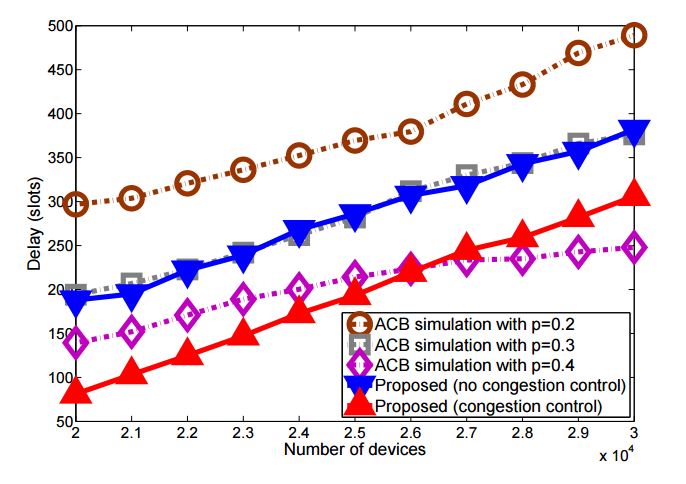
\includegraphics[width=.4\linewidth]{figures/delay1.png}
          \caption{Thesis}
          \label{fig:sub1}
        \end{subfigure}%
        \begin{subfigure}{.5\textwidth}
          \centering
          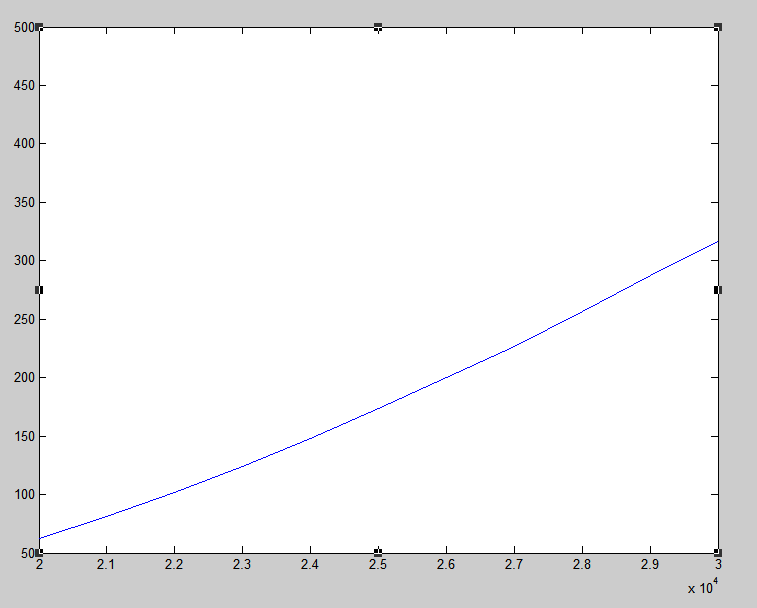
\includegraphics[width=.4\linewidth]{figures/delay2.png}
          \caption{simulation}
          \label{fig:sub2}
        \end{subfigure}
        \caption{Access delay}
        \label{fig:test}
    \end{figure}
\end{frame}

\begin{frame} {Problem in Machine Type Communication} 
    \begin{itemize}
        \item {Different service like real-time health service can not tolerance with the environment with high access delay and failure of access}
        \item \textbf{Alleviate the Radio Access Network overload}
        \begin{itemize}    
            \item[-]{ellvate the access success probability}
        \end{itemize}
        \begin{itemize}    
            \item[-]{reduce access delay}
        \end{itemize}
    \end{itemize}
\end{frame}

\begin{frame}{Random Access Procedure - intro}
    \begin{figure}[t]
        \centering
        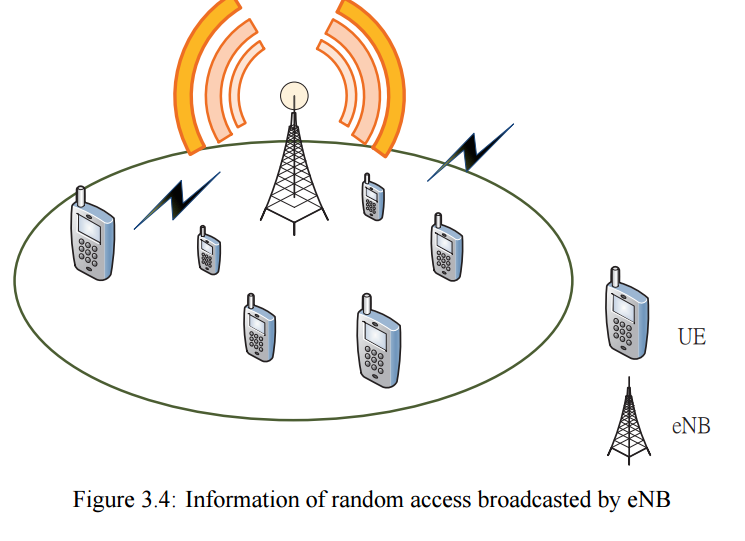
\includegraphics[width=0.9\textwidth]{figures/envir.png}
        \setbeamerfont{caption}{size=\tiny}
    \end{figure}
\end{frame}

\begin{frame}{Random Access Procedure - intro}
    \begin{itemize}
        \item{Random Access Procedure is triggered when}
        \begin{itemize}    
            \item[-]{Initial access from RRC\_IDLE}
            \item[-]{Handover}
            \item[-]{DL data arrival during RRC\_CONNECTED requiring random access procedure}
        \end{itemize}
    \end{itemize}
\end{frame}

\begin{frame}{Terms}
    \begin{itemize}
        \item{RACH - Random Access Channel}
        \begin{itemize}    
            \item[-]{time-frequency resource blocks repeats in the system periodically}
        \end{itemize}
        \item{Preamble}
        \begin{itemize}    
            \item[-]{A set of codes called preambles, which shared by all users in their random access}
        \end{itemize}
    \end{itemize}
\end{frame}

\begin{frame}{Random Access Procedure - two type}
    \begin{figure}[t]
        \centering
        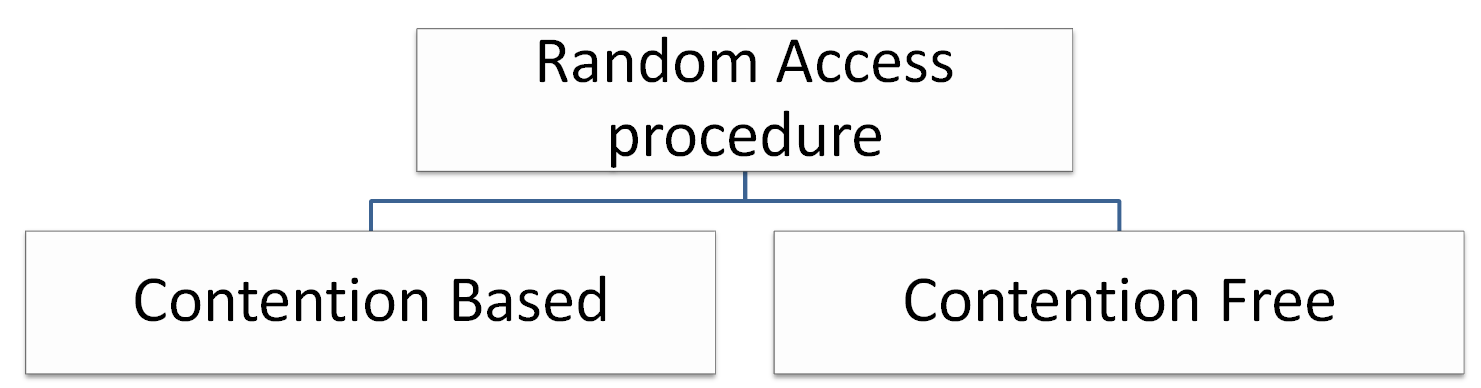
\includegraphics[width=0.9\textwidth]{figures/content.png}
        \setbeamerfont{caption}{size=\tiny}
    \end{figure}
\end{frame}
\begin{frame}{Random Access Procedure - illustration}
    \begin{figure}[t]
        \centering
        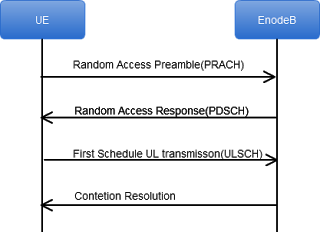
\includegraphics[width=0.8\textwidth]{figures/rap.png}
        \setbeamerfont{caption}{size=\tiny}
    \end{figure}
\end{frame}

\begin{frame}{Congestion of Random Access Procedure}
    \begin{itemize}
        \item {Lets assume two UEs send same RACH preamble at same time in step 1}
        \item {Same message will be received by two UEs in step 2}
        \item {In step 3 eNodeB may be able to receive Msg3 from only one UE or none of them due to interference}
        \item {In step 4 the UE which does not receive Msg4 from eNodeB will back-off after expiration of RACH specific timers. Possibility is also that none of them receive Msg4}

    \end{itemize}
\end{frame}

\begin{frame}{ACB - Access Class Barring}
    \begin{itemize}
        \item{eNB broadcast an access probability $p$ and a limit time $\tau$}
        \item{UE will generate a random value $q$, if $q \leq p$, UE can start the Random Access Procedure}
        \item{if not, UE have to wait for $\tau$ to retry}
    \end{itemize}
\end{frame}

\begin{frame}{MTC backoff}
    \begin{itemize}
        \item{When there is collision in Random Access Procedure, UE will wait for a backoff time to retry}
        \item{Use the backoff time to release loading on Random Access Channel}
    \end{itemize}
\end{frame}

\begin{frame}{Random Access Procedure - flow chart}
    \begin{figure}[t]
        \centering
        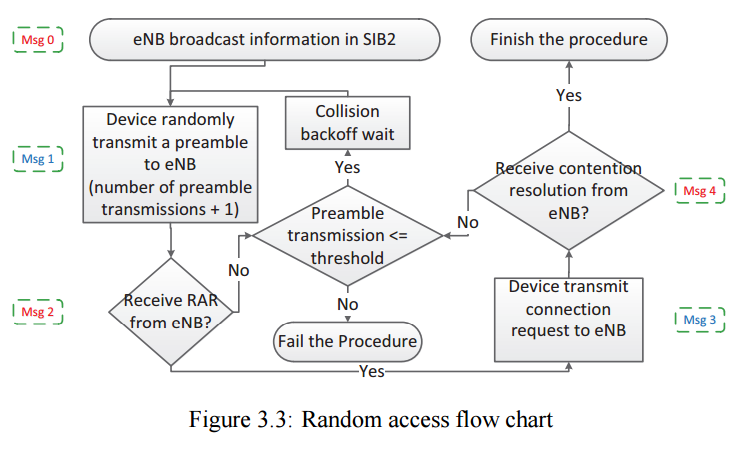
\includegraphics[width=1\textwidth]{figures/flow.png}
        \setbeamerfont{caption}{size=\tiny}
    \end{figure}
\end{frame}


%%%%%%%%%%%%%%%%%%%%%%%%%%%%%%%%%%%%%%%%%%%%%%%%%%%%%%
%%%%%%%%%%%%%%%%%%%%%%%%%%%%%%%%%%%%%%%%%%%%%%%%%%%%%%

\section{Solutions}
\begin{frame} {Papers} 
    \begin{itemize}
        \item {Retransmission-based Access Class Barring for RAN overload control in Machine Type Communications}\cite{RACB}
        \item {Efficient LTE Access with Collision Resolution for Massive M2M Communications} \cite{TRAO}
        \item {Adaptive RACH Congestion Management to Support M2M Communication in 4G LTE Networks} \cite{ARC}
        \item {D-ACB: Adaptive Congestion Control Algorithm for Bursty M2M Traffic in LTE Networks} \cite{DACB}
    \end{itemize}
\end{frame}

\begin{frame}{Solution from these papers}
    \begin{itemize}
        \item {Retransmission-based Access Class Barring for RAN overload control in Machine Type Communications}\cite{RACB}
        \begin{itemize}
            \item [-]{Classify into several groups by the number of retransmission. Each group were assigned a weight which means the proportion of RACH resource they get.}
           \item [-]{The way to control the proportion of RACH resource is dynamic change their ACB factor}
        \end{itemize}
    \end{itemize}
\end{frame}

\begin{frame}{Solution from these papers}
    \begin{itemize}
        \item {Efficient LTE Access with Collision Resolution for Massive M2M Communications}
        \begin{itemize}
            \item [-]{Proposed a collision resolution algorithm. The algorithm use q-ary tree spliting to split the set of avaliable preable}
            \item [-]{Revise MSG4 to make UE next contention attempt use the sub-set of available preamble on dedicate RAO(random access oppo
            rtunity)}
        \end{itemize}
    \end{itemize}
\end{frame}

\begin{frame}{Solution from these papers}
    \begin{figure}[t]
        \centering
        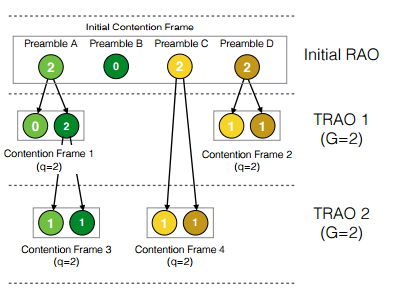
\includegraphics[width=0.9\textwidth]{figures/TRAO.png}
        \setbeamerfont{caption}{size=\tiny}
    \end{figure}
\end{frame}

\begin{frame}{Solution from these papers}
    \begin{itemize}
        \item {Adaptive RACH Congestion Management to Support M2M Communication in 4G LTE Networks}
        \begin{itemize}
            \item [-]{With several known algorithm for congestion control, and seperate congestion situation in three level.}
            \item [-]{Propose an algorithm ``ARC'', to apply the best congestion control algo to correspond congestion level.}
        \end{itemize}
    \end{itemize}
\end{frame}

\begin{frame}{Solution from these papers}
    \begin{itemize}
        \item {D-ACB: Adaptive Congestion Control Algorithm for Bursty M2M Traffic in LTE Networks}
        \begin{itemize}
            \item [-]{Proposed a ``D-ACB'' algorithm to adaptively update the ACB factor}
            \item [-]{Use available information (e.g. number of success preamble transmissions, number of available preambles...) to derive ${E[C_{M,p}]}$: average number of preambles experiencing collisions in the RACH}
            \item [-]{and use ${E[C_{M,p}]}$ can derive the improved ACB factor}
        \end{itemize}
    \end{itemize}
\end{frame}
%%%%%%%%%%%%%%%%%%%%%%%%%%%%%%%%%%%%%%%%%%%%%%%%%%%%%%
%%%%%%%%%%%%%%%%%%%%%%%%%%%%%%%%%%%%%%%%%%%%%%%%%%%%%%
\section{Conclusion}
\begin{frame}{Difference between this papers}
    \begin{itemize}
        \item {The work in \cite{RACB} and \cite{DACB} both discuss with how to adjust ACB factor}
        \begin{itemize}
            \item [-]{These two paper are using the same parameter ``ACB'' to alleviate the Radio Access Network}
            \item [-]{but \cite{RACB} is more focused on the access success probability, so it's hard to integrate to gain better result}
        \end{itemize}
        \item {\cite{TRAO} and \cite{DACB} both concern in how to decrease access delay}
        \begin{itemize}
            \item [-]{Combine the perspective between these two, might gain better result}
        \end{itemize}
    \end{itemize}
\end{frame}
%%%%%%%%%%%%%%%%%%%%%%%%%%%%%%%%%%%%%%%%%%%%%%%%%%%%%%
%%%%%%%%%%%%%%%%%%%%%%%%%%%%%%%%%%%%%%%%%%%%%%%%%%%%%%
\section{References}
\calcreferencespagetotal % Calc your References Page total number
\begin{frame}[allowframebreaks]{References}
    \fontsize{9pt}{13}\selectfont
    \bibliographystyle{IEEEtran}
    \bibliography{IEEEabrv,Citation}
\end{frame}

%%%%%%%%%%%%%%%%%%%%%%%%%%%%%%%%%%%%%%%%%%%%%%%%%%%%%%
%%%%%%%%%%%%%%%%%%%%%%%%%%%%%%%%%%%%%%%%%%%%%%%%%%%%%%
\section{}

\begin{frame}
    \centering
    \Large{Thanks for Your Attentions}
\end{frame}

\end{document}
